\documentclass[14pt]{extarticle}
\usepackage[utf8]{inputenc}
\usepackage[spanish]{babel}
\usepackage{enumerate}
\usepackage{graphicx}
\usepackage{listings}
\usepackage{graphicx}
\usepackage{ dsfont }
\usepackage{caption}
\usepackage{subfigure}
\usepackage{ amssymb }
\usepackage[hidelinks]{hyperref}
\usepackage[vmargin=3cm,hmargin=2cm]{geometry}

\title{Entendiendo la Teoría de Nudos mediante la Simulación y la Informática Gráfica.}

\begin{document}
\newtheorem{teo}{Teorema}[section]

\maketitle

\tableofcontents

\newpage
\section{Teoría de nudos. }\label{PrimerTema}

\subsection{Motivación y primeras definiciones.}
  ¿Alguna vez has visto una cuerda con nudos y te has preguntado si podrías deshacerlos sin necesidad de romper la cuerda? ¿Te has planteado si algo tan usual como los nudos pueden estar presentes en áreas esenciales para la vida? Es más, ¿cuál fue el motivo inicial para estudiar dicha teoría de nudos? Quizás te sorprendan las respuestas pero antes de descubrirlo, veamos que se entiende formalmente por un nudo.\\
  
\underline{\textbf{Definición:}}\\
 Un \textbf{nudo} es una curva cerrada en $\mathds{R}^{3}$ que no tiene auto-intersecciones.\\

Podemos representar un nudo en el plano visualizando su proyección. Como hay muchas formas de representar un mismo nudo, podremos tener diferentes proyecciones que representen al mismo nudo. 
 Algunos ejemplos básicos son los siguientes:
 
  \begin{figure}[h!]
  	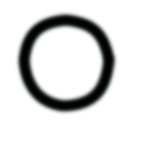
\includegraphics[width=2cm]{1.jpg}
  	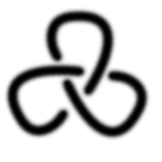
\includegraphics[width=2cm]{3f.png} 
  	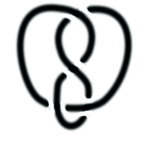
\includegraphics[width=2cm]{fig8.jpg}
  	\centering
  	\caption{De izquierda a derecha: nudo trivial, nudo trébol, nudo de ocho.}
  	\label{uno} 
  \end{figure}
  
  Podemos ver en ellos una serie de cruces. En concreto en el nudo trébol tenemos 3 cruces y el nudo de ocho tenemos 4 cruces. El nudo trivial destaca por no tener ningún cruce. \\
  
    \underline{\textbf{Definición:}}\\
     Un \textbf{enlace} es una o más curvas cerradas disjuntas en $\mathds{R}^{3}$. Cada una de sus curvas recibe el nombre de componente.\\
     Por ejemplo, el siguiente enlace tiene dos componentes:
  \begin{figure}[h!]
  	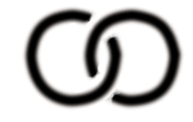
\includegraphics[width=2.7cm]{enlace.png}
  	\centering
  	\label{dos} 
  \end{figure}
    \newpage
    Por tanto, podemos ver un nudo como un caso particular de enlace en el que sólo tenemos una componente.\\
    
  Una de las cuestiones más interesantes en la teoría de nudos es la siguiente: \\
  ¿Dada un nudo, o alguna proyección suya, podremos saber si se trata del nudo trivial?. A lo largo de este proyecto trataremos de dar respuesta, en parte, a dicha cuestión.\\
  
  Esta rama de la topología de baja dimensión destaca por su gran interés en áreas como:
  \begin{enumerate}
  	\item Química: En el siguiente apartado veremos que la teoría de nudos nace en este área.
  	\item Biología: se descubrieron los anudamientos en las moléculas de ADN. 
  	\item Criptografía: 
  	//TENGO QUE COMPLETAR LAS ÁREAS!!!!!!!!!!!!!!
  \end{enumerate}
 
  \newpage
\subsection{Sobre su historia.}
En el siglo XIX, ciertos físicos escoceses se preguntaban por la estructura de los átomos.\\
Estos científicos tomaron como base la teoría de Descartes, que afirmaba que el \textit{éter} era un fluido que ocupaba todo el espacio y transmitía la luz (éter lumínico), para desarrollar su modelo del átomo. \\
Aunque dichos físicos conocían la existencia de los elementos y que estaban formados por átomos, no conocían la propia estructura de los átomos. \\

Científicos como Peter Guthrie Tait y Willian Thomson llegaron a la teoría de que los átomos se concebían como vórtices, que podríamos ver como remolinos tubulares, en dicho fluido. Estos vórtices se encontraban anudados y en función del tipo de anudamiento darían lugar a un tipo de elemento u otro.\\
De este modo se plantearon que los diferentes nudos corresponderían a los diferentes elementos de la naturaleza. De acuerdo con la teoría, si conociésemos todos los nudos posibles, crearíamos la tabla de elementos que reemplazaría la tabla periódica actual. \\

Para hacernos una idea más clara, para Willian Thomson el nudo trébol podría corresponder con el átomo de helio, el nudo de ocho con el átomo de oxígeno....\\

Numerosos científicos contribuyeron a dicha teoría intentando crear la tabla de nudos pero a finales de este mismo siglo, Michelson-Morley demostró que el éter lumínico no existía y por tanto la teoría de los átomos de vórtice fue descartada. \\

Tras este hecho, la teoría de nudos perdió su interés hasta que fue objeto de estudio en Topología a principios del siglo XX.


\newpage
\subsection{Componiendo nudos.}
Supongamos que tenemos dos proyecciones J y K de nudos. Podemos definir un nuevo nudo a partir de ellos eliminando un arco de cada una de las proyecciones y conectando los 4 extremos finales de dos en dos mediante otros arcos de modo que no se añadan ni eliminen cruces.\\
A este nudo resultante le llamaremos \textbf{composición} de los dos nudos y se denotará como \textbf{J\#K}. A los nudos originales J y K les llamaremos \textbf{nudos factores}. \\

Por ejemplo, consideremos como nudos factores el nudo trébol y el nudo de ocho. 
  \begin{figure}[h!]
  	\subfigure[J]{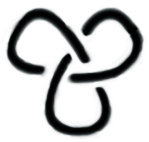
\includegraphics[width=2.5cm]{conexion1.jpg}} 
  	\subfigure[K]{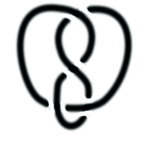
\includegraphics[width=2.5cm]{fig8.jpg}}
  	\centering
  	\caption{Nudo trébol y nudo de ocho.}
  	\label{comp1} 
  \end{figure}
  
Haciendo la suma conexa de ambos nudos obtenemos el nudo composición:
  \begin{figure}[h!]
  	\subfigure[Haciendo la composición]{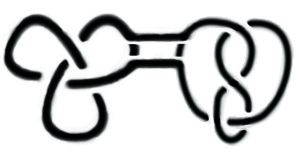
\includegraphics[width=7cm]{conexion2.jpg} }
  	\subfigure[J\#K]{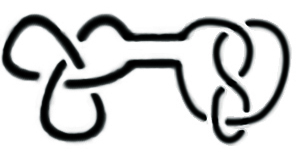
\includegraphics[width=7cm]{conexion3.jpg}}
  	\centering
  	\caption{Composición de nudo trébol y nudo de ocho.}
  	\label{comp2} 
  \end{figure}
  
  
  El nudo trivial es un elemento identidad para la suma conexa: si hacemos la composición de un nudo cualquiera J con el nudo trivial, vamos a obtener el propio nudo J. Por ejemplo, seguimos considerando J como el nudo trébol y el nudo trivial como K. \\
   \begin{figure}[h!]
   	\centering
   	\subfigure[J]{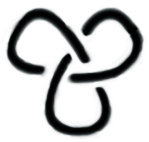
\includegraphics[width=2.5cm]{conexion1.jpg} }
   	\subfigure[K]{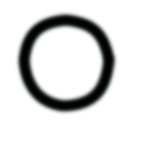
\includegraphics[width=2.5cm]{1.jpg}}
   	\caption{Nudo trébol y nudo trivial.}
   	\label{comp3} 
   \end{figure}
   
  Su suma conexa nos seguiría dando el nudo factor J, es decir, el nudo trébol.\\
   
      \begin{figure}[h!]
      	\subfigure[Haciendo la composición]{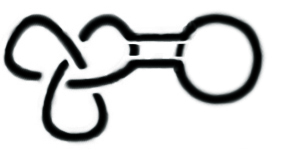
\includegraphics[width=8cm]{conexion4.jpg} }
      	\subfigure[J\#K]{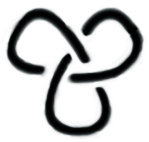
\includegraphics[width=4cm]{conexion1.jpg}}
      	\centering
      	\caption{Composición de nudo trébol y nudo trivial.}
      	\label{comp4} 
      \end{figure}
  
 \underline{\textbf{ Definición:}}\\
 Diremos que un \textbf{nudo es primo} si no puede ser expresado como la suma conexa de dos nudos, a menos que uno de ellos sea el nudo trivial. \\
 
\underline{ \textbf{ Definición:}}\\
 Diremos que un \textbf{nudo es compuesto} si no es el nudo trivial ni es un nudo primo.\\
  
  Por ejemplo, los nudos trébol y nudo de ocho de la figura \ref{comp1} son nudos primos mientras que el nudo de la figura \ref{comp2} es un nudo compuesto. \\ 
  
  Hay una gran variedad de nudos primos. Cualquier nudo puede ser expresado singularmente como suma conexa de nudos primos. En la siguiente tabla podemos ver los diferentes nudos primos que tienen menos de 8 cruces.\\
        \begin{figure}[h!]
        	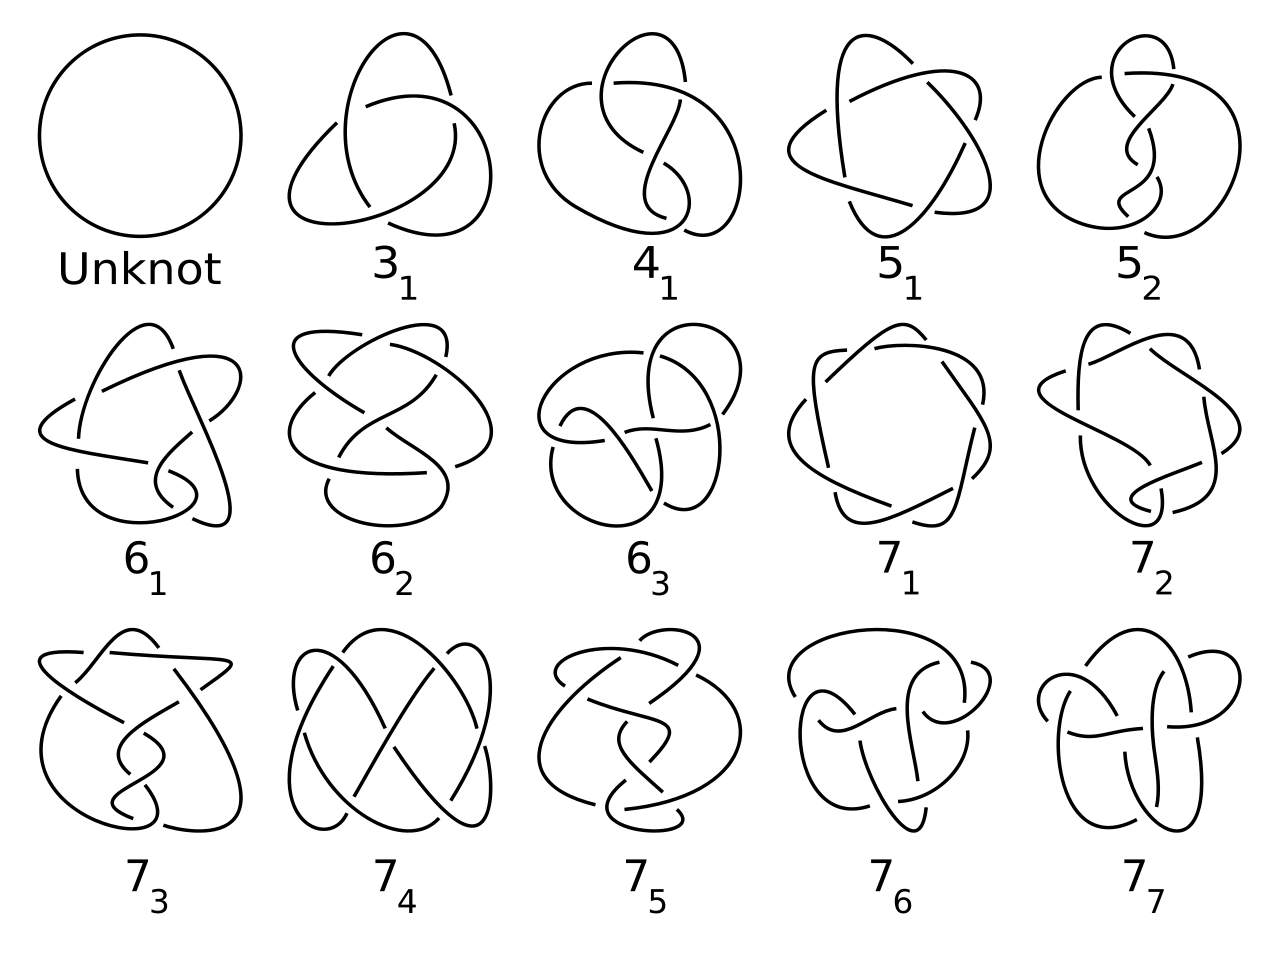
\includegraphics[width=14cm]{tableknot.png}
        	\centering
        	\caption{Composición de nudo trébol y nudo trivial.}
        	\label{comp6} 
        \end{figure}
  
  
  
    
    Finalmente, es importante destacar el hecho de que la elección que hacemos de los arcos que eliminamos de cada uno de los nudos factores afecta al nudo composición. Por tanto, es posible construir dos nudos composición diferentes a partir del mismo par de nudos factores. Veamos esta idea con más detalle, para ello necesitamos:\\
    
   \underline{\textbf{ Definición:}}\\
   \textbf{ Un nudo orientado} es un nudo al que se le ha asignado una orientación, es decir, es un nudo que dispone de una dirección de viaje sobre él mismo. Esta orientación se indica mediante flechas en la proyección. \\
   
   \underline{\textbf{ Definición:}}\\
   \textbf{ Un nudo es invertible} si es equivalente a sí mismo con la orientación opuesta. \\
   
      El problema de determinar si un nudo cualquiera es o no invertible no es para nada trivial.\\
   
   Como ejemplo de nuevo invertible nos podemos encontrar el nudo trébol.
      \begin{figure}[h!]
      	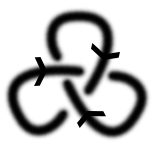
\includegraphics[width=3cm]{3fcon1.png}
      	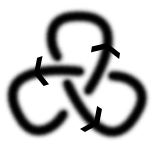
\includegraphics[width=3cm]{3fcon2.png}
      	\centering
      	\caption{Ambas orientaciones del nudo trébol.}
      	\label{comp5} 
      \end{figure}
   
   Sean los dos nudos factores J y K a los que se asignamos una orientación. Tendremos dos formas posibles de hacer la composición: conectar con las orientaciones emparejadas o no emparejadas. \\
   Todas las composiciones de los nudos cuyas orientaciones emparejan al componer, darán el mismo nudo composición. Todas las composiciones de los nudos cuyas orientaciones no emparejan al componer, también darán el mismo nudo composición. Sin embargo, es posible que la composición de los nudos cuyas orientaciones emparejen no de lugar al mismo nudo que haciendo la composición de los nudos cuyas orientaciones no emparejen. Serán el mismo si uno de los nudos factores es invertible.\\
   
   Veamos un caso en el que la composición de dos mismos factores, genera nudos diferentes. Consideramos el siguiente nudo:
         \begin{figure}[h!]
         	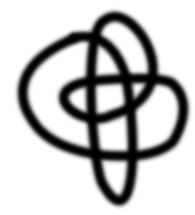
\includegraphics[width=3cm]{817.png}
         	\centering
         	\caption{Nudo factor J y K.}
         	\label{comp7} 
         \end{figure}
   Si componemos el nudo consigo mismo conectando las orientaciones emparejadas y desemparejadas obtenemos nudos que no son equivalentes. Lo podemos comprobar visualmente con la Figura \ref{comp8}.
   
         \begin{figure}[h!]
         	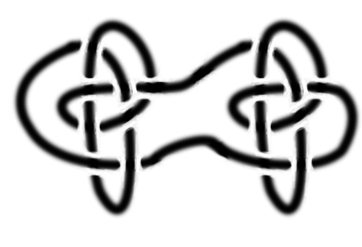
\includegraphics[width=6.5cm]{817def1.png}
         	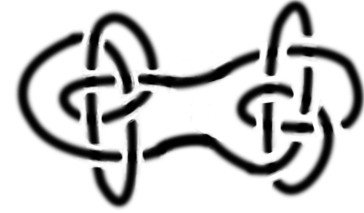
\includegraphics[width=6.5cm]{817def2.png}
         	\centering
         	\caption{Las composiciones no son equivalentes.}
         	\label{comp8} 
         \end{figure}
 
    
   
\subsection{Equivalencia de nudos: movimientos de Reidemeister.}
Dos nudos K1 y K2 serán equivalentes (K1 $\thicksim$ K2) si podemos distorsionar uno de ellos en el otro sin hacer ningún corte. A esta distorsión se le conoce como isotopía ambiente. \\

Una deformación de la proyección de un nudo se llama isotopía plana si se deforma el plano de proyección como si estuviese hecho de goma.\\
Con más precisión definimos una \textbf{isotopía plana} de las proyecciones P1 y P2 de nudos como la aplicación continua $F: \mathds{R}^{2}$ x $[0,1] \rightarrow \mathds{R}^{2}$ tal que $F_{0}=identidad$, $F_{1}(P1) = P2$ y $F_{t}$ es un homeomorfismo $\forall t$.\\

Los movimientos de Reidemeister que vamos a ver a continuación nos permiten cambiar la proyección de un nudo de modo que se cambie la relación entre los cruces pero que no cambie el nudo al que representa la proyección. Cada uno de estos movimientos es una isotopía:\\

	\textbf{Primer movimiento de Reidemeister.}\\
En cualquier zona de la proyección nos permite añadir o eliminar un giro tal y como vemos en la figura \ref{movi1}.\\

  \begin{figure}[h!]
  	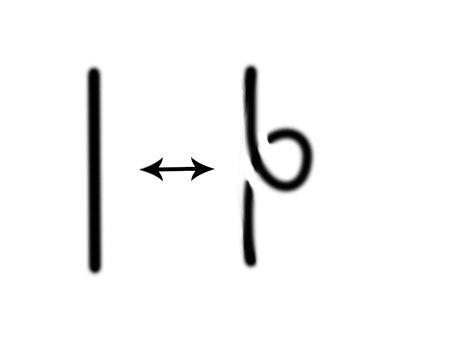
\includegraphics[width=7.2cm]{movi1.png}
  	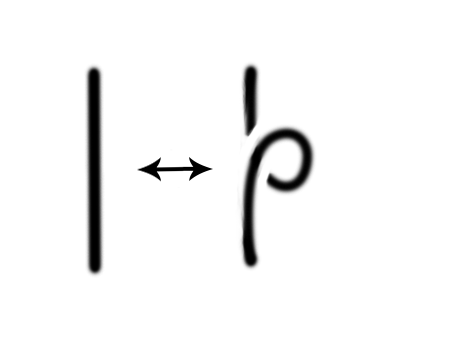
\includegraphics[width=7.2cm]{movi2.png}
  	\centering
  	\caption{Primer movimiento Reidemeister.}
  	\label{movi1} 
  \end{figure}
  
	\textbf{Segundo movimiento de Reidemeister.}\\
Nos permite añadir o eliminar dos cruces del nudo como se ve en la figura \ref{movi2}.\\

    \begin{figure}[h!]
    	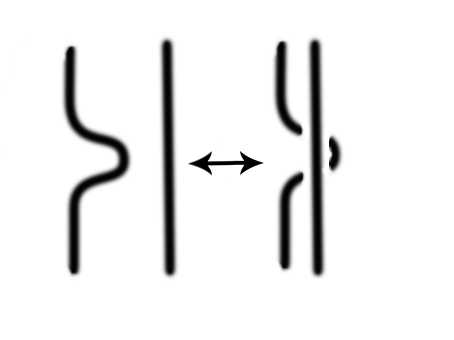
\includegraphics[width=7.5cm]{movi3.png}
    	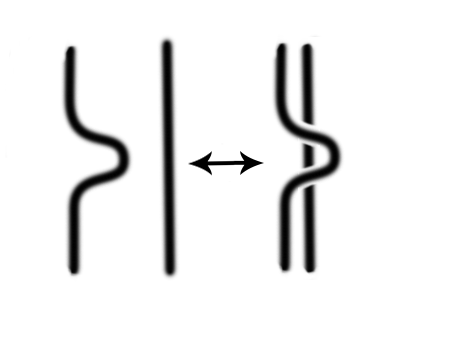
\includegraphics[width=7.5cm]{movi4.png}
    	\centering
    	\caption{Segundo movimiento de Reidemeister.}
    	\label{movi2} 
    \end{figure}
    
	\textbf{Tercer movimiento de Reidemeister.}\\
Nos permite deslizar una hebra del nudo de un lado de un cruce al otro lado del cruce. Veamos la figura \ref{movi3} para aclarar la idea.
      \begin{figure}[h!]
      	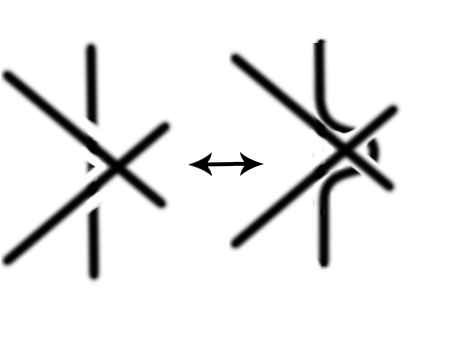
\includegraphics[width=7.5cm]{movi5.png}
      	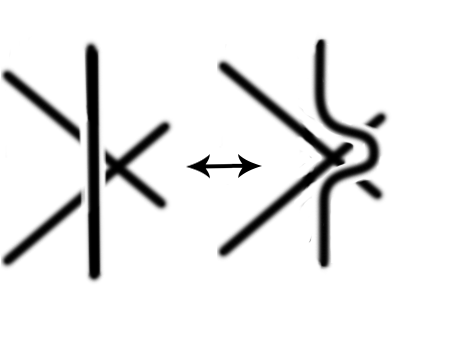
\includegraphics[width=7.5cm]{movi6.png}
      	\centering
      	\caption{Tercer movimiento de Reidemeister.}
      	\label{movi3} 
      \end{figure}
  

\begin{teo} \textbf{Teorema de Reidemeister.} Sean P1 y P2 las proyecciones que representan a dos nudos K1 y K2, respectivamente. Entonces, K1 $\thicksim$ K2 si, y solo si, P1 y P2 están conectados por una secuencia finita de movimientos de Reidemeister e isotopías planas.
\end{teo}
//PENDIENTE DEMOSTRACIÓN. NO ESTÁ EN LOS LIBROS.\\
//PONER EJEMPLO VISUAL DE UNA SECUENCIA DE MOVIMIENTOS. \\

Gracias a dicho teorema podremos estudiar si dos proyecciones representan el mismo nudo. Para ello tendremos que encontrar una secuencia de movimientos de Reidemeister que nos lleve de una proyección a la otra. Sin embargo, este proceso puede no tener el número de movimientos intermedios limitado por lo que no tiene mucho sentido implementarlo.\\
 
 Aunque este teorema no nos permita ver de una forma cómoda la equivalencia entre dos nudos en la práctica (por la fuerte complejidad) si que nos permite obtener una conclusión esencial:\\
 
 Si una propiedad de un nudo no cambia al aplicarle cualquiera de estos tres movimientos de Reidemeister, entonces esta propiedad no va a cambiar por muchas deformaciones que se le hagan al nudo. En definitiva, si un nudo cumple cierta propiedad y otro nudo no la cumple, esos nudos no podrán ser equivalentes. Incidiremos en esta idea en la siguiente Sección \ref{seccion5}.
 
  

\newpage
\subsection{Algunos invariantes.}\label{seccion5}
Suponga que cierto día ha ido a trabajar con su portátil fuera de casa y se lo ha dejado olvidado. Cuando te das cuenta, vuelves a buscarlo pero ya no está. Pasan unos días y un amigo te comenta que se ha encontrado un portátil con $x$ número de puertos, procesador $y$ y modelo $z$.\\

Es claro que si alguna de esas características no fuese la de tu portátil, tendrías claro que no es el tuyo. Pero resulta que tu portátil tiene exactamente las mismas características. Piensas que tal vez sea tu portátil pero no tienes garantía de que realmente lo sea. \\

Algo similar, aplicado a nudos, es lo que vamos a tratar de ver en esta sección. ¿Dadas dos proyecciones, podremos decir que representan al mismo nudo? Vamos a tratar de estudiar ciertos invariantes sobre los nudos. Al igual que ocurría con el caso del portátil, si dos proyecciones tienen valores de un invariante distintos podremos decir que no representan al mismo nudo. Sin embargo, si ambos tienen valores de un invariante iguales no podremos saber si se trata del mismo nudo. Tendremos que estudiar otros invariantes de nudos. \\

¿Y si estudiamos una gran cantidad de invariantes de dos proyecciones y siempre toman los mismos valores?¿Podremos garantizar que son equivalentes? La respuesta es clara, no. Tendremos que analizar en mayor detalle las proyecciones, pero puede ser que no lleguemos a obtener un conclusión definitiva. \\

    
Por tanto, el estudio de invariantes de los nudos nos va a permitir saber si dos nudos pueden ser (destacamos, que no quiere decir que lo sean) o no son equivalentes.\\


Antes de ver algunos de los invariantes de nudos más conocidos y útiles vamos a dar una definición formal de lo que se conoce como un invariante:\\

\underline{\textbf{Definición:}} \\
Un \textbf{invariante} de un nudo (o de un enlace) es una propiedad que no cambia cuando el nudo sufre deformaciones en el espacio. \\



\begin{center}
	\textbf{Número de componentes:}
\end{center}
Es uno de los invariantes de enlaces más sencillos que nos podemos encontrar y que ya hemos comentado ligeramente en las secciones anteriores.\\

Cada componente de un enlace es una curva disjunta del mismo. En la Figura \ref{inv1} vemos un enlace con dos componentes. 
  \begin{figure}[h!]
  	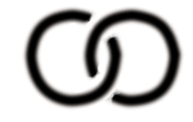
\includegraphics[width=2.7cm]{enlace.png}
  	\centering
  	\caption{Enlace con dos componentes.}
  	\label{inv1} 
  \end{figure}
  
Al aplicarle a un enlace cualquier transformación no se le puede añadir ni eliminar ninguna componente. De modo que este invariante no nos va a permitir comparar nudos, pues todo nudo tiene una sola componente. \\

\bigskip
\begin{center}
	\textbf{Crossing number:}
\end{center}
Sea un nudo K. Su \textbf{crossing number} es el menor número de cruces que se encuentra en cualquier proyección del nudo. Se denota como $c(K)$. \\

Esto nos lleva a deducir el nudo K tendrá como mínimo c(K) cruces por muchas transformaciones que se haga a sus proyecciones.\\

Aunque es un invariante sencillo de visualizar, no es fácil de obtener: puede ser que al estudiar muchas proyecciones de un nudo pensemos que su número de cruces es $n$, sin embargo puede existir otra proyecciones del nudo que no conocemos con menor número de cruces. Por este motivo, no vamos a trabajar posteriormente con este invariante.\\

Para dejarlo más claro vamos a ver un ejemplo.\\
Consideramos la siguiente proyección de cierto nudo. Podemos pensar que el número de cruces del nudo sería 4 (ver los 4 cruces de la figura a //PONER ENLACE). Sin embargo, esta proyección es equivalente a la proyección que vamos en la figura b //PONER ENLACE, que tiene como número de cruces el valor 3. Por tanto, el número de cruces del nudo, que es el nudo trébol, es 3. 

//HACER IMAGENES!!!!!!!!!!!!!!!!!!!!!!!!!!!!!!!!!!    


\begin{center}
	\textbf{Tricolorabilidad:}
\end{center}
Para definir este invariante de enlaces, tenemos que conocer unos conceptos previos:\\
Entendemos por undercrossing y overcrossing a un recorrido en el cruce de la proyección de un nudo que nos lleva por encima o por debajo en el cruce. Veamos la siguiente imagen donde queda representado:\\
\\HACER IMAGEN!!!!!!!!!!!!!!!!!!!!!!!!!!!!!!!!!!

\underline{\textbf{Definición:}}\\
Una\textbf{ hebra }de una proyección de un enlace es una región de cuerda del enlace que va desde un undercrossing a otro undercrossing con sólo overcrossings en su recorrido.\\ 

\underline{\textbf{Definición:}}\\
Una proyección de un enlace es tricolorable si cada una de las hebras de la proyección puede ser coloreada con uno de tres colores diferentes de modo que en cada cruce o los 3 colores se junten o se junte un sólo color. En este caso diremos que el enlace es \textbf{tricolorable}. 

\begin{teo}
	La tricolorabilidad se perserva mediante movimientos de Reidemeister.
\end{teo}
//DEMOSTRACION EN KNOTS, MOLECULES....

Haciendo uso de este invariante podemos demostrar que el nudo trivial y el nudo trébol no son equivalentes, es decir, son topológicamente distintos. Esto se debe a que el nudo trébol es tricolorable pero el nudo trivial no lo es. Podemos verlo en la siguiente imagen:\\
//PONER IMAGEINES DEL TRIVIAL Y DEL TREBOL COLOREADO!!!!!!!!!!!!!!!!


Este hecho confirma que existe al menos un nudo distinto del nudo trivial. Es más, todo nudo que sea tricolorable será distinto del nudo trivial.\\
Sin embargo, este invariante no es muy potente en el sentido de que sólo clasifica los enlaces en tricolorables y no tricolorables y sólo podremos afirmar que dos proyecciones representan a diferentes nudos si una de ellas es tricolorable y la otra no lo es.   



\begin{center}
	\textbf{Unkotting number:}
\end{center}

\begin{center}
	\textbf{Cruces positivos y negativos:}
\end{center}

\subsection{Notación de nudos.}
\subsection{Tipos y ejemplos de nudos.}




 



\end{document}
